\chapter[Estado do arte]{Estado do Arte\label{estado_do_arte}}

Neste capítulo explicarase como funciona a internacionalización e localización con GNU Gettext. Ademais analizaremos as diferentes alternativas que existen no mercado como ferramentas de asistencia a tradución e as características que cada unha incorpora. O final faremos un resumo das características que empregan os programas CAT\footnote{Computer Assisted Translation}.

\section{Internacionalización e localización con GNU Gettext}
Gettext é un sistema para a internacionalización e localización amplamente usado en entornos UNIX. Conta con varías implementacións, sendo a primeira de Sun Microsystems no ano 1990. A implementación máis usada é a que GNU liberou no ano 1995. Pese ser unha solución antiga, é a día de hoxe a mellor que se pode atopar no mercado.

Para internacionalizar un programa con GNU Gettext non empregaremos as cadeas de texto directamente como podería ser no seguinte programa de exemplo:

\begin{lstlisting}[language=C,label=some-code,caption=helloworld.c (Sen Internacionalizar)]
#include <stdio.h>

int
main ()
{
    printf ("Hello World!");
}
\end{lstlisting}

En lugar diso chamaremos a unha función especial que proporciona Gettext de nome \lstinline{gettext()} pero que é máis empregada a través do seu alias \lstinline{_()}. Ademais configuraremos o programa para que colla a tradución do idioma que queiramos. Desta forma o programa anterior quedaría:

\begin{lstlisting}[language=C,label=some-code,caption=helloworld.c]
#include <stdio.h>
#include <locale.h>
#include <libintl.h>

#define _(str) gettext(str)

#define

int
main ()
{
    setlocale (LC_ALL, "");
    bindtextdomain ("helloworld", "/usr/local/share/locale");
    textdomain ("helloworld");

    printf (_("Hello World!"));
}
\end{lstlisting}

A función \lstinline{gettext()} é a encargada de substituír a cadea orixinal pola tradución. Non obstante vemos que debemos configurar algunhas cousas antes de poder chamar á función.

En primeiro lugar debemos establecer a linguaxe que queremos empregar no programa. Para iso usamos a función \lstinline{setlocale()}. O primeiro argumento da función determina que parte do locale actual queremos modificar. Entre outras podemos atopar:

\begin{itemize}
    \item \textbf{LC\_ALL.} Queremos cambiar todo.
    \item \textbf{LC\_ADDRESS.} Queremos cambiar a forma de formatar os enderezos.
    \item \textbf{LC\_MESSAGES.} Os mensaxes do programa.
    \item \textbf{LC\_NUMERIC.} O formatado das cantidades non monetarias
    \item \textbf{LC\_TIME.} O formatado de datas e horas.
\end{itemize}

Por último especificamos o código de idioma ou no caso de empregar a cadea baleira empregamos os valores das variables de entorno.

Os códigos de idioma empregan a normativa ISO 639 polo que son da forma $$language[\_territory][.codeset][@modifier]$$ Por exemplo o código do galego empregando codificación UTF-8 é \lstinline{gl\_ES.UTF-8}.

Ademais debemos indicarlle o programa onde ten que atopar as traducións. Para iso empregamos a función \lstinline{bindtextdomain()} que liga un nome de dominio a unha ruta dentro do sistema e a función \lstinline{textdomain()} que lle indica o programa cal é o nome de dominio que debe empregar. Un dominio é un conxunto de cadeas que se empregan nunha parte determinada dun programa. Cada dominio debe ter un nome de dominio único dentro dun programa.

Con estes parámetros Gettext xa é capaz de atopar as traducións que no caso do programa anterior atoparíanse en \emph{/usr/local/share/locale/gl/LC\_MESSAGES/helloworld.mo}.

Unha vez que internacionalizamos o nosos programa debemos traducir as cadeas. Pero para traducir as cadeas debemos extraelas antes do código fonte. Para iso empregaremos a utilidade \emph{xgettext}. Empregando as opcións adecuadas obtemos o seguinte ficheiro:

\begin{lstlisting}[label=some-code,caption=helloworld.pot]
# SOME DESCRIPTIVE TITLE.
# Copyright (C) YEAR THE PACKAGE'S COPYRIGHT HOLDER
# This file is distributed under the same license as the PACKAGE package.
# FIRST AUTHOR <EMAIL@ADDRESS>, YEAR.
#
#, fuzzy
msgid ""
msgstr ""
"Project-Id-Version: PACKAGE VERSION\n"
"Report-Msgid-Bugs-To: \n"
"POT-Creation-Date: 2014-11-12 19:24+0100\n"
"PO-Revision-Date: YEAR-MO-DA HO:MI+ZONE\n"
"Last-Translator: FULL NAME <EMAIL@ADDRESS>\n"
"Language-Team: LANGUAGE <LL@li.org>\n"
"Language: \n"
"MIME-Version: 1.0\n"
"Content-Type: text/plain; charset=CHARSET\n"
"Content-Transfer-Encoding: 8bit\n"

#: helloworld.c:14
#, c-format
msgid "Hello World!"
msgstr ""
\end{lstlisting}

Os ficheiros Gettext coa estensión \emph{POT} trátanse de plantillas xenéricas para todos os idiomas. Para obter o arquivo especifico para o noso idioma debemos empregar a ferramenta \emph{msginit} coa que obteremos un ficheiro similar a este:

\begin{lstlisting}[label=some-code,caption=helloworld.po (Sen Traducir)]
# Galician translations for HELLOWORLD package.
# Copyright (C) 2014 THE HELLOWORLD COPYRIGHT HOLDER
# This file is distributed under the same license as the ch package.
# Marcos Chavarría Teijeiro <chavarria1991@gmail.com>, 2014.
#
msgid ""
msgstr ""
"Project-Id-Version: ch 01\n"
"Report-Msgid-Bugs-To: \n"
"POT-Creation-Date: 2014-11-12 19:24+0100\n"
"PO-Revision-Date: 2014-11-12 19:54+0100\n"
"Last-Translator: Marcos Chavarría Teijeiro <chavarria1991@gmail.com>\n"
"Language-Team: Galician\n"
"Language: gl_ES\n"
"MIME-Version: 1.0\n"
"Content-Type: text/plain; charset=ISO-8859-1\n"
"Content-Transfer-Encoding: 8bit\n"

#: helloworld.c:14
#, c-format
msgid "Hello World!"
msgstr ""
\end{lstlisting}

Desta forma obtemos un ficheiro Gettext PO que é o ficheiro que temos que editar. Traducindo o arquivo obtemos algo como isto:

\begin{lstlisting}[label=lst:translated_example,caption=helloworld.po (Traducido)]
# Galician translations for HELLOWORLD package.
# Copyright (C) 2014 THE HELLOWORLD COPYRIGHT HOLDER
# This file is distributed under the same license as the HELLOWORLD package.
# Marcos Chavarría Teijeiro <chavarria1991@gmail.com>, 2014.
#
msgid ""
msgstr ""
"Project-Id-Version: HELLOWORLD 1.0\n"
"Report-Msgid-Bugs-To: \n"
"POT-Creation-Date: 2014-11-12 19:24+0100\n"
"PO-Revision-Date: 2014-11-12 19:54+0100\n"
"Last-Translator: Marcos Chavarría Teijeiro <chavarria1991@gmail.com>\n"
"Language-Team: Galician\n"
"Language: gl_ES\n"
"MIME-Version: 1.0\n"
"Content-Type: text/plain; charset=ISO-8859-1\n"
"Content-Transfer-Encoding: 8bit\n"

#: helloworld.c:14
#, c-format
msgid "Hello World!"
msgstr "Ola Mundo!"
\end{lstlisting}

Antes de poder empregar o ficheiro no noso programa temos que compilalo. Para iso empregamos a utilidade msgfmt ca que obtemos o ficheiro helloworld.mo. Se movemos o ficheiro o directorio adecuado (o que especificamos en \lstinline{textdomain()}) o noso programa xa estará localizado.

%http://www.gnu.org/software/libc/manual/html_node/Locating-gettext-catalog.html

\subsection{Ficheiros Gettext PO}
Como xa dixemos antes os ficheiros PO son os ficheiros que temos que editar para localizar o noso programa. Primeiro dicir que se trata ficheiros de texto plano e que polo tanto podemos editar con calquera editor de ficheiros de texto plano. Non obstante, o ideal é empregar algunha ferramenta que nos facilite a tarefa como pode ser unha ferramenta CAT.

As súas principais características son:

\paragraph{Soporte de plurais}
Algo que pode parecer trivial como o soporte de plurais deixa de selo cando consideramos que non todos as linguaxes do mundo empregan dous plurais. A lingua eslovaca, por exemplo, conta con tres formas de plural de forma que o plural faise diferente para 1, 3 e 5 elementos.

Gettext representa a forma de plural de cada linguaxe con unha cadea da seguinte forma: $$nplurals=n; plural=exp;$$ Onde $n$ representa o número de plurais da linguaxe e $exp$ a expresión para calcular cando debemos empregar cada forma. Por exemplo a forma plural do galego representase como $nplurals=2; plural=(n != 1);$. Isto é que temos 2 plurais e que so se emprega a forma singular cando o número de elementos é igual a $1$.

No código fonte para que GetText escolla a tradución adecuada temos que empregar a función \lstinline{ngettext}. Esta función recibe como parámetros a cadea orixinal en singular, a cadea orixinal en plural e o número de elementos. No seguinte fragmento de código temos un exemplo:

\begin{lstlisting}[language=C,caption=Plurais en GetText (Código Fonte).]
[...]
    printf (ngettext ("We have %d car.", "We have %d cars.", n), n);
[...]
\end{lstlisting}

A cadea do ficheiro PO correspondente o código anterior pódese ver no seguinte fragmento de código. Vemos como temos unha entrada \lstinline{msgstr} por cada plural. Desta forma o plural número $0$ corresponde os singular é o plural número $1$ correspondese coa primeira forma do plural.

\begin{lstlisting}[caption=Plurais en GetText (Ficheiro PO).]
#: helloworld.c:19
#, c-format
msgid "We have %d car."
msgid_plural "We have %d cars."
msgstr[0] "Temos %d coche."
msgstr[1] "Temos %d coches."
\end{lstlisting}


\paragraph {Marcado de traducións difusas}
Permítese marcar certas traducións como difusas de forma que o tradutor indica que non estar seguro de que dita tradución sexa correcta. Se marcásemos a tradución \emph{"Hello World!"} como difusa o ficheiro PO tería o seguinte aspecto:

\begin{lstlisting}[label=some-code,caption=Ficheiro POT con comentario.]
[...]
#: helloworld.c:15
#, c-format
#, fuzzy
msgid "Hello World!"
msgstr ""
[...]
\end{lstlisting}

\paragraph {Formato das traducións}
Os ficheiro PO permite indicar se as cadeas a traducir teñen un formato determinado. Por exemplo a cadea do exemplo no Fragmento de Código \ref{lst:translated_example} pódese ver que ten o flag \lstinline{c-format} debido a que é parte dunha sentencia printf e podería levar indicadores de formato da forma \lstinline{%s}.

\paragraph {Cabeceira con metadatos}
Existe unha cadea especial nos documentos Gettext PO. Trátase da cadea baleira que serve para almacenar metadatos do ficheiro. No fragmento de código \ref{lst:translated_example} podemos ver istos metadatos. Algúns dos metadatos existentes son:

\begin{itemize}
    \item \textbf{Project-Id-Version.} Nome único para o proxecto deste arquivo de tradución.
    \item \textbf{Report-Msgid-Bugs-To.} Ligazón onde reportar errores nas cadeas orixinais ou para pedir contexto para facer a tradución.
    \item \textbf{POT-Creation-Date.} Data de creación do ficheiro POT.
    \item \textbf{PO-Revision-Date.} Data da última actualización das traducións.
    \item \textbf{Last-Translator.} Nome e enderezo de correo electronico do último traductor.
    \item \textbf{Language-Team.} Enderezo de correo eléctronico do equipo de traductores.
    \item \textbf{Language.} Linguaxe do ficheiro expresada coa codificación ISO 639.
    \item \textbf{Content-Type.} Tipo MIME do ficheiro, que será sempre \lstinline{text/plain} e codificación dos caracteres.
    \item \textbf{Plural-Forms.} Expresión da forma plural empregada.
\end{itemize}

Ademais destes campos, nos comentarios, gárdanse os nomes de todas as persoas que contribuíron a esta tradución.

\paragraph{Gardado dos orixes das cadeas}
Gettext almacena para cada cadea en que lugares do código aparece esta. O cal pode ser moi interesante para implentar a previsualización das traducións. Por exemplo no Fragmento de Código~\ref{lst:translated_example} vemos como a cadea \emph{"Hello World!"} pode atoparse na liña 14 do ficheiro \lstinline{helloworld.c}.

\paragraph{Comentarios dos programadores}
É unha función moi importante xa que en moitas ocasións nas linguaxes a mesma palabra empregase como verbo ou como nome polo que en ocasións é importante incorporar un contexto para esa tradución. Para facer isto é necesario simplemente poñer un comentario no programa antes de empregar a cadea. Por exemplo no seguinte fragmento de código:

\begin{lstlisting}[language=C,caption=Tradución con comentario.]
[...]
    // Translators: We are just waving the world.
    printf (_("Hello World!"));
[...]
\end{lstlisting}

Estamos engadindo un comentario a cadea \emph{"Hello World!"}. O ficheiro POT resultado tería a forma:

\begin{lstlisting}[label=some-code,caption=Ficheiro POT con comentario.]
[...]
#. Translators: We are just waving the world.
#: helloworld.c:15
#, c-format
msgid "Hello World!"
msgstr ""
[...]
\end{lstlisting}


\paragraph{Comentarios dos tradutores}
A biblioteca permite que os tradutores comenten as cadeas. Engadindo un comentario á cadea \emph{"Hello World!"}, o ficheiro PO tería o seguinte aspecto:

\begin{lstlisting}[caption=Ficheiro PO con comentario.]
[...]
# This is a note from translators.
#: helloworld.c:15
#, c-format
msgid "Hello World!"
msgstr ""
[...]
\end{lstlisting}

\section{Ferramentas CAT do mercado}

Nesta sección analizaremos algunhas das ferramentas de asistencia a tradución existentes. Veremos as características que incorporan estes programas así como estudar a súa interface de usuario.

\subsection{GTranslator}
GTranslator é a aplicación oficial do proxecto GNOME para a asistencia a tradución. Este aplicativo so permite a tradución de arquivos GNU Gettext. As característica máis destacables deste programa son a posibilidade de abrir varios ficheiros en diferentes lapelas, soporte de memorias de tradución, perfiles para diferentes tradutores, edición dos comentarios dos ficheiros .po e un sistema de plugins que permite estender a ferramenta.

\begin{figure}[h]
    \centering
    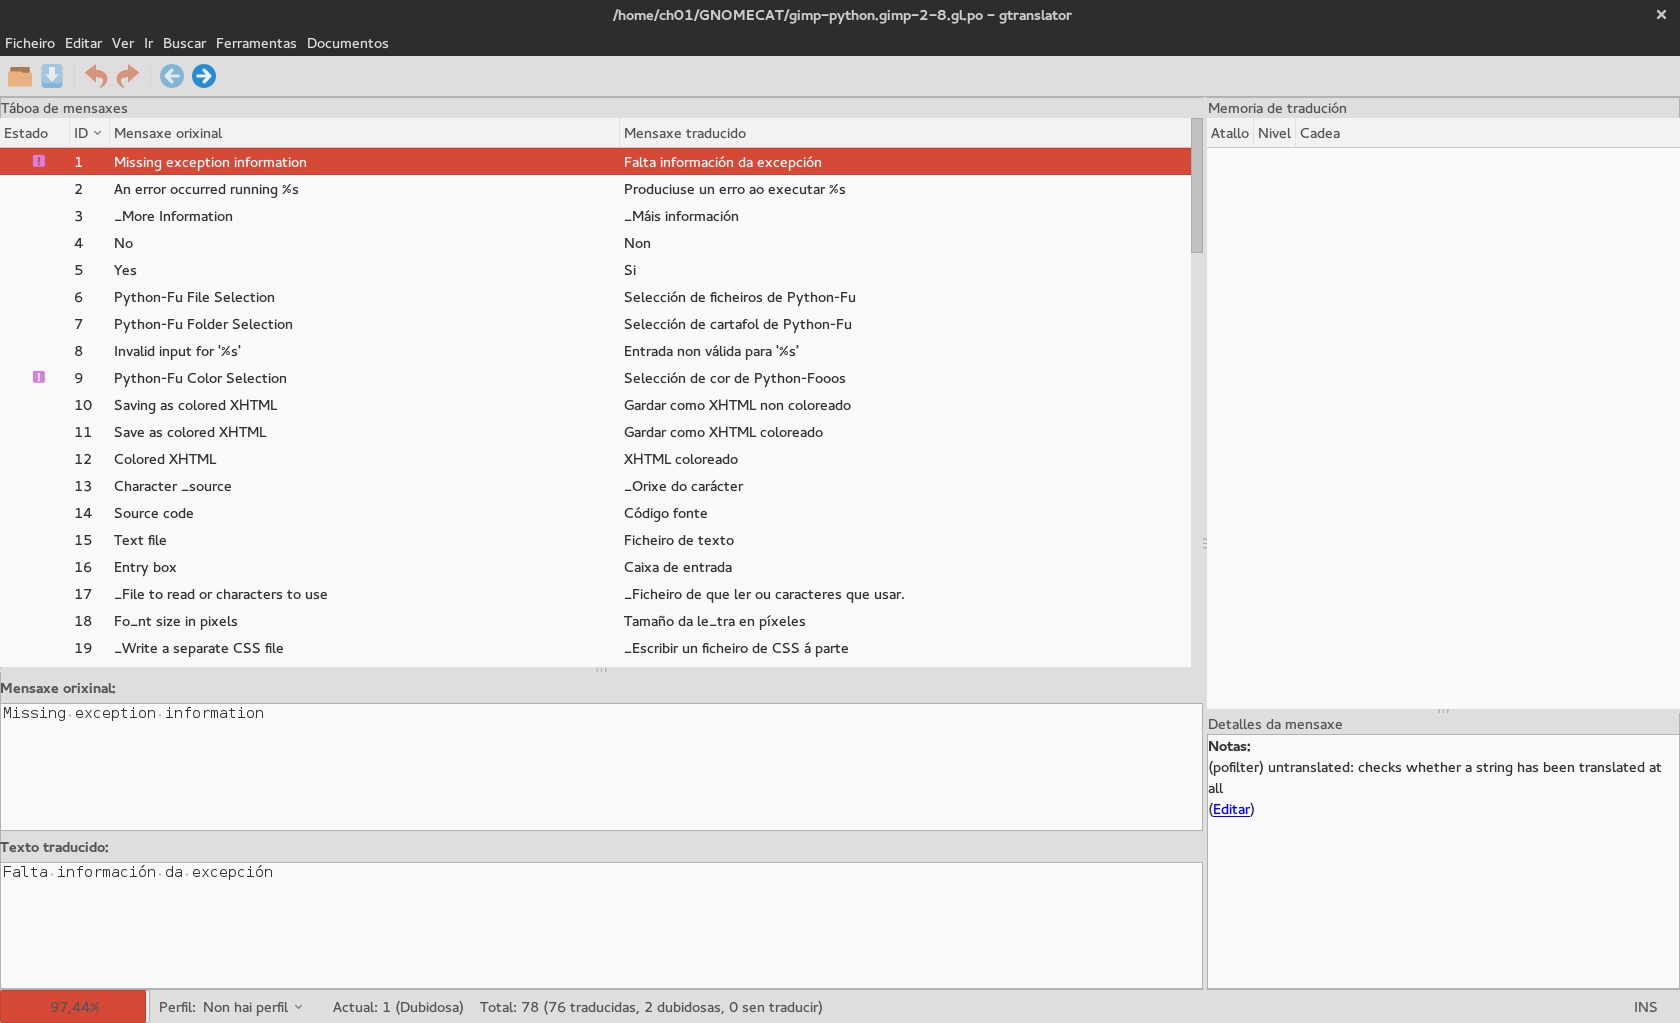
\includegraphics[width=\textwidth]{img/captura_gtranslator.png}
    \caption[Interface de GTranslator]{Interface de GTranslator}
    \label{fig:gtranslator}
\end{figure}

En canto a interface, como podemos ver na Figura~\ref{fig:gtranslator}, a parte máis importante do programa é a a lista de mensaxes. Abaixo desta lista temos un panel onde se pode editar cada mensaxe e a súa dereita a memoria de tradución. A disposición dos elementos desta interface é configurable xa que permite mover e ampliar cada un dos módulos. O programa tamén incorpora atallos de teclado que permiten moverse polo documento e seleccionar cada elemento da memoria de tradución.

Este programa pese a ser o aplicativo oficial de GNOME é moi pouco usado. As razóns disto son a ausencia dunha característica chave que o diferencie doutras ferramentas do mercado, a presencia de fallas importantes que afectan a usabilidade e a ausencia dun mantedor que resolva estes problemas.

\subsection{Lokalize}
Lokalize é o programa oficial para o soporte a tradución en KDE. Foi escrita dende cero empregando a tecnoloxía de KDE Platform 4 e baseándose no código de KBabel. As súas características máis destacables son, o soporte para ficheros GNU Gettext e o formato QT TS entre outros; a xestión de proxectos incorporando unha vista que permite ver un resumo de cada ficheiro dentro do proxecto; uso de memorias de tradución e de glosarios; comprobación da ortografía e vista previa das traducións a partir de scripts feitos polo usuario.

\begin{figure}[h]
    \centering
    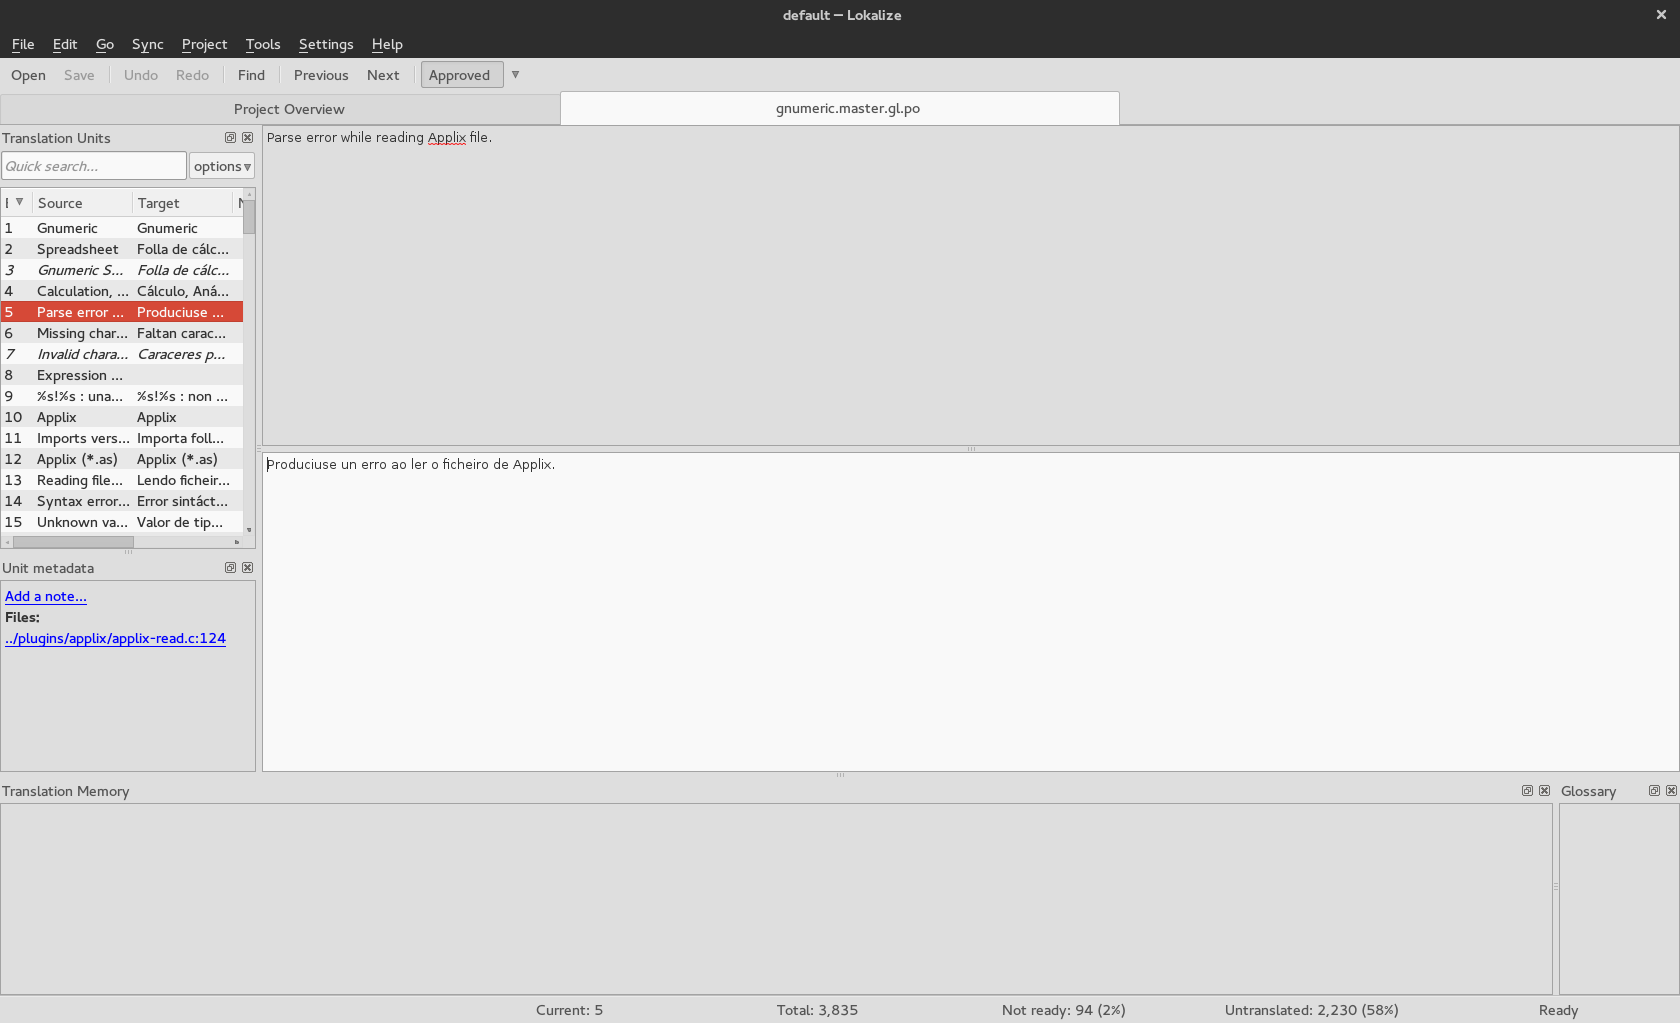
\includegraphics[width=\textwidth]{img/captura_lokalize.png}
    \caption{Interface de Lokalize}
    \label{fig:lokalize}
\end{figure}

En canto a interface, o programa permite abrir varios ficheiros cada un na súa lapela. Como se pode ver na Figura~\ref{fig:lokalize}, a vista de tradución está centrada no panel de edición, onde aparecen tanto a cadea orixinal como a cadea a traducir. Na columna da esquerda podemos ver a lista de cadeas onde se amosan os primeiros caracteres da cadea orixinal e da tradución e o estado desta tradución. Ademais tamén se pode ver o contexto da tradución, engadir un novo comentario e ver en que ficheiros estaba dita tradución. Por último tamén podemos ver na parte inferior a memoria de tradución e o glosario.

\subsection{Virtaal}

Virtaal é unha ferramenta CAT creada por Translate House\footnote{Compañía que surxiu a partir dunha comunidade de tradutores de Sudáfrica e que está especializada na creación de ferramentas e bibliotecas para axudar a tradución.} As características máis destacables son a incorporación de suxestión a tradución, comprobación da calidade das tradución e, sobretodo, a capacidade de abrir unha gran variedade de formatos a través da biblioteca Translate Toolkit.

\begin{figure}[h]
    \centering
    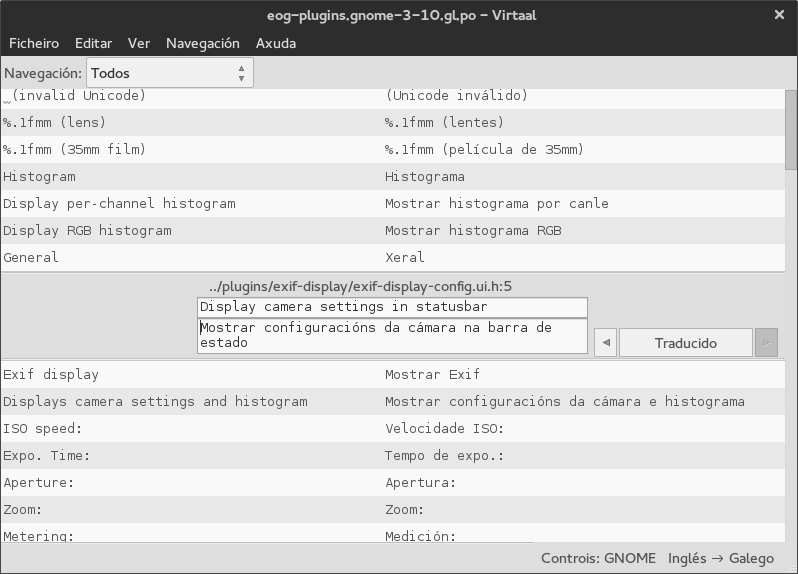
\includegraphics[width=\textwidth]{img/captura_virtaal.png}
    \caption{Interface de Virtaal}
    \label{fig:virtaal}
\end{figure}

Como se pode ver na Figura~\ref{fig:virtaal}, a interface é minimalista e moi centrada na tradución. A diferencia dos casos anteriores, trátase dunha interface fixa e que integra a lista das mensaxes coa edición da propia mensaxe. Tamén se indican posibles fallos que poidan ter a tradución, como falta de puntos o final, ausencia de marcadores de formato, etc.

\subsection{OmegaT}
Ferramenta CAT lanzada no ano 2001 e pensada fundamentalmente para tradutores profesionais. Ten soporte para o uso de memoria de tradución, glosario, tradución directa entre outras cousas. Destaca a gran cantidade de formatos que pode empregar.

\begin{figure}[h]
    \centering
    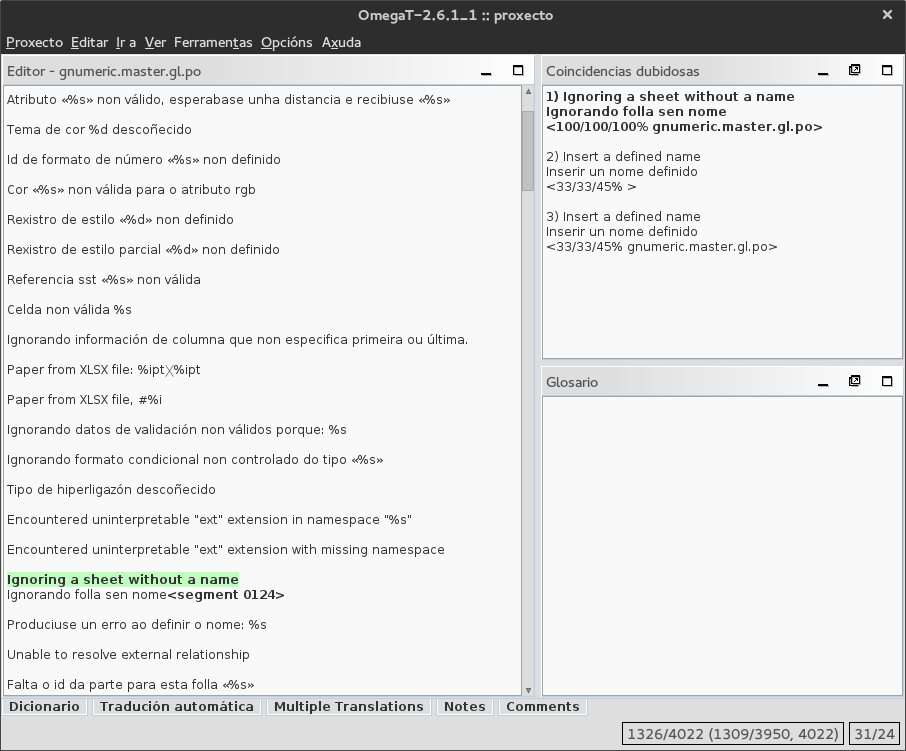
\includegraphics[width=\textwidth]{img/captura_omegat.png}
    \caption{Interface de OmegaT}
    \label{fig:omegat}
\end{figure}

A interface de OmegaT dista bastante do resto de programas. Como amosa a Figura~\ref{fig:omegat} non existe o concepto de lista de mensaxes traducir. O documento amosase como unha sucesión de cadea e se facemos clic encima dunha, permitiranos traducila. Trátase dun programa moi usado para a tradución tanto profesional como amateur.

\subsection{Google Translation Toolkit}
É a ferramenta CAT desenvolvida por Google e lanzada no ano 2008. A diferencia dos aplicativos analizados anteriormente, esta trátase unha solución puramente web. Entre as súas principais características encontrase a posibilidade de facer tradución automática empregando Google Translator, o uso de memorias de tradución compartidas, glosarios, soporte de etiquetas HTML entre outros e atallos de teclado. Ten soporte para varios formatos como ficheiros PO, documentos de Microsoft Word, de LibreOffice ou mesmo artigos da Wikipedia.

\begin{figure}[h]
    \centering
    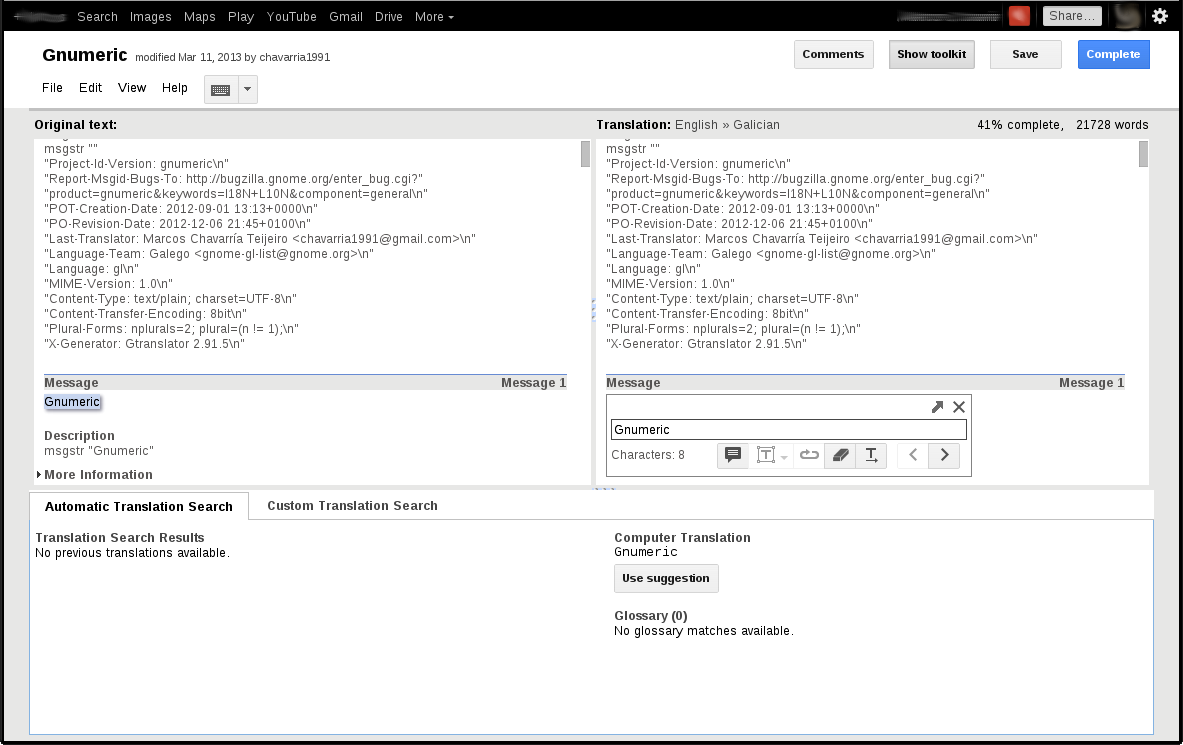
\includegraphics[width=\textwidth]{img/captura_googletranslationtoolkit.png}
    \caption{Interface de Google Translation Toolkit}
    \label{fig:translatetoolkit}
\end{figure}

Como se pode ver na Figura~\ref{fig:translatetoolkit}, na interface misturase a lista de cadeas co cadro de edición das mesmas. Ademais empregando unha interface semellante a do resto de ferramentas ofimáticas de Google, temos botóns para autocompletar tags e para avanzar a seguinte tradución. Aínda que foi pensado para a tradución colaborativa de documentos de ONGs e artigos da Wikipedia, na actualidade emprégase maioritariamente para a tradución de proxectos comerciais.


\subsection{Transifex}
Trátase dunha plataforma que xurdiu a partir dun proxecto do Google Summer of Code do ano 2007 que pretendía crear unha plataforma online máis amigable que o Damned Lies de GNOME que naquel momento tamén empregaba Fedora unha distribución de GNU/Linux. Trátase dunha solución de pago con plans que van dende os 19 a os 300 dólares. Non obstante os proxectos de código aberto poden usar o servizo de forma gratuíta e dispón de un período de mostra 30 días. As súas principais características son a posibilidade de descargar o documento e volvelo a subir para poder traducilo con outra ferramenta CAT, editor online, memoria de tradución e unha API que permite integralo con outros servizos. Ademais tamén soporta unha gran variedade de formatos entre os que se atopan os ficheiros PO, DTD de Mozilla ou XML entre outros.

\begin{figure}[h]
    \centering
    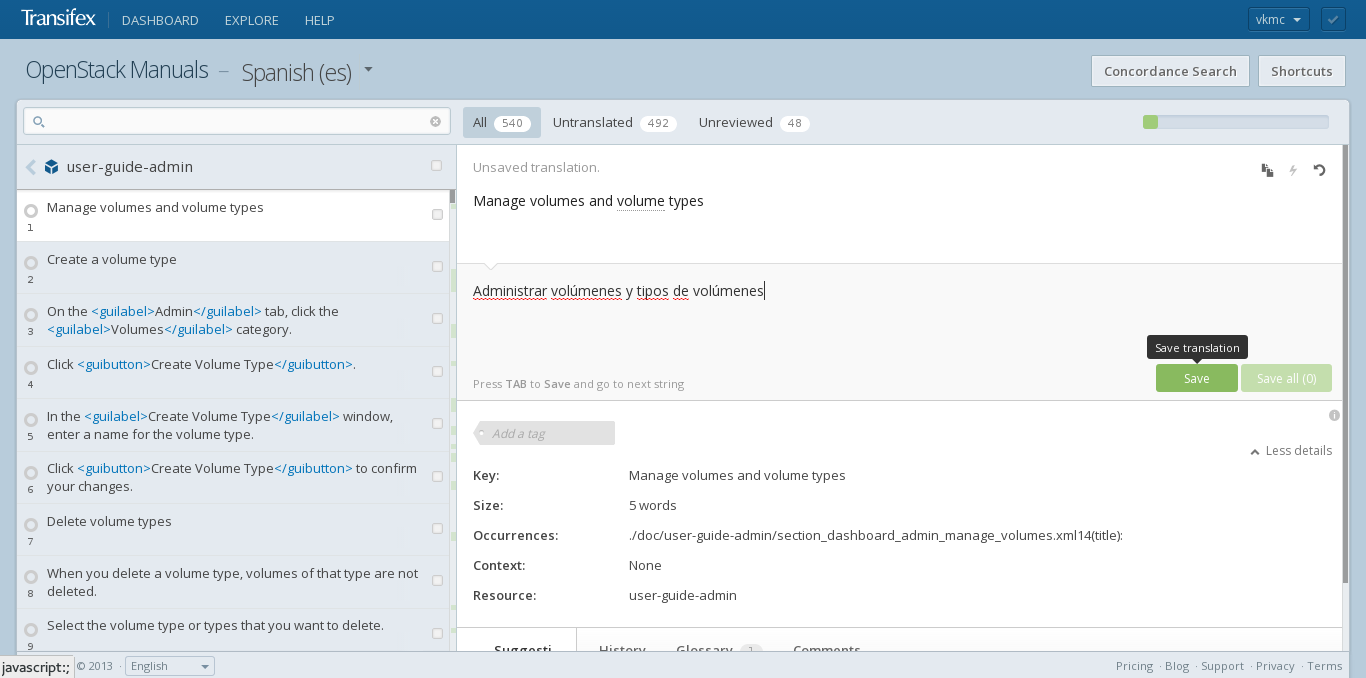
\includegraphics[width=\textwidth]{img/captura_transifex.png}
    \caption{Interface de Transifex}
    \label{fig:transifex}
\end{figure}

A interface de trasifex, como ser pode ver na Figura~\ref{fig:transifex} separa a lista de cadeas do cadro de edición. No cadro de edición temos a posibilidade de consultar a memoria de tradución ou o glosario. O programa tamén incorpora resaltado de sintaxe.

\subsection{Outras ferramentas}
Existen moitas máis ferramentas CAT no mercado. De feito, segundo unha enquisa \cite{article:2006survey} elaborada polo Imperial College London a cerca de 900 tradutores profesionais de 54 países diferentes, os únicos programas de todos os anteriores que aparecen citados é o OmegaT que conta con un 7\% de usuarios. As ferramentas máis usadas son ferramentas para Microsoft Windows e ferramentas con licencias privativas e usualmente moi caras. Algunhas destas ferramentas son TRADOS, Wordfast, DejaVu SDLX ou STAR Transit. Na Figura~\ref{fig:enquisa2006} podemos ver unha gráfica coas ferramentas máis empregadas segundo este estudio.

\begin{figure}[h]
    \centering
    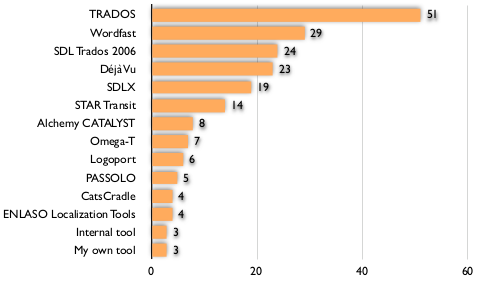
\includegraphics[width=0.7\textwidth]{img/grafico_uso_cat_enquisa2006.png}
    \caption{Ferramentas CAT máis empregadas segundo \cite{article:2006survey}.}
    \label{fig:enquisa2006}
\end{figure}

Hai que ter tamén en conta que se trata dun estudio bastante antigo polo que algunhas das ferramentas analizadas aínda non existían. Por exemplo a enquisa cita a ferramenta KBabel, que é a ferramenta de KDE na que está baseada Lokalize, pero con menos dun 2\% de usuarios.


\section{Características xenéricas das ferramentas CAT}

Algunhas das características que aparecen de forma recurrente en todas as ferramentas analizadas son as seguintes:

\subsection{Memoria de Tradución}
Unha memoria de tradución é unha base de datos composta de textos orixinais acompañados das súas traducións. Estes textos almacénanse en segmentos onde a separación entre segmentos ven dada por signos de puntuación ou o cambio de parágrafo, sendo esta última forma a máis frecuente.

A principal función dunha memoria de tradución e a extracción de coincidencias totais ou parciais. Os programas que teñen esta característica buscan na base de datos un segmento que coincida de forma exacta ou parcial coa cadea que se está a traducir e mostrase este segmento como suxerencia. Xunto coa suxerencia tamén se amosa o grado de cercanía entre a cadea a traducir e a cadea da memoria de tradución.

Existe un formato estándar de compartición de memorias de tradución de nome Translation Memory eXchange (TMX) e plataformas online que almacenan gran cantidade de cadeas e polo tanto hai máis posibilidade de obter unha mellor coincidencia. O software Amagama creado por Translate House, os creadores de Virtal, é un exemplo de memoria de tradución online.

\subsection{Glosario}
Un glosario é unha base de datos de termos xunto con unha ou varias traducións aceptadas. Diferenciase da memoria de tradución en que so se proporcionan a tradución a termos e non a cadeas completas. De igual forma que no caso das memorias de tradución, existe un formato estándar de para a compartición de glosarios de nome TermBase eXchange (TBX) e plataformas online para almacenar os glosarios.


\subsection{Previsualización}
As funcións de previsualización permítenlle ó tradutor ver como vai quedar a cadea traducida no programa final.

Os programadores e deseñadores fan as interfaces tendo en conta a lingua orixinal e non ningunha das traducións polo que se unha tradución é moito máis longa ca orixinal pode verse mal no programa final.

Para conseguir esta característica pódense empregar varias técnicas:

\begin{itemize}
  \item \textbf{Programa orixinal.} Esta técnica que se pode empregar en calquera cadea consiste en compilar o ficheiro PO e executar o programa final con ese ficheiro PO. Desta poderemos ver como queda a nosa tradución para o usuario final. A desvantaxe deste método consiste en que teremos que saber en que parte do programa se emprega a cadea que queremos previsualizar. Este método é empregado por Lokalize que permite a definición de scripts para a previsualización de cadeas.

  \item \textbf{Renderizado de interfaces de usuario en XML.} Nas bibliotecas de interfaces modernas existe a posibilidade de definir interfaces en ficheiros XML e despois renderizalas. Neste caso as cadeas a traducir van nestes arquivos e sería posible renderizar esta interface coa tradución que estamos a realizar. Este método aínda que si que amosaría a pantalla onde aparece a cadea actual, so é válido para as cadeas que proveñen destes ficheiros XML e non as definidas da forma tradicional. Un exemplo deste método pódese ver na rede no aplicativo Deckard\footnote{\href{http://deckard.malizor.org/}{deckard.malizor.org}} que permite ver as traducións de aplicativos de GNOME.
\end{itemize}


\subsection{Tradución Directa}
A tradución de cadeas de forma automática empregando algoritmos deseñados a tal proceso e que empregan grandes bases de datos aloxadas, xeralmente en internet. Tanto Google como Microsoft teñen os seus produtos corporativos que fan traducións e existen alternativas libres como OpenTrad ou Apertium. Estas traducións aínda que validas soen ser de baixa calidade polo que necesitan unha revisión.
